\chapter{Measurements}
\label{chapter:measurements}
    
    Executing the previously described tests, extensive results were gained on all tested platforms.
    The following chapter presents the results obtained.
    Apart from a description, causes for specific results are identified and their implications  discussed.

    
    \section{OpenStack's Resource Consumption}
    \label{section:evaluation_consumption}
    
        \begin{figure}[ht]
          \centering
          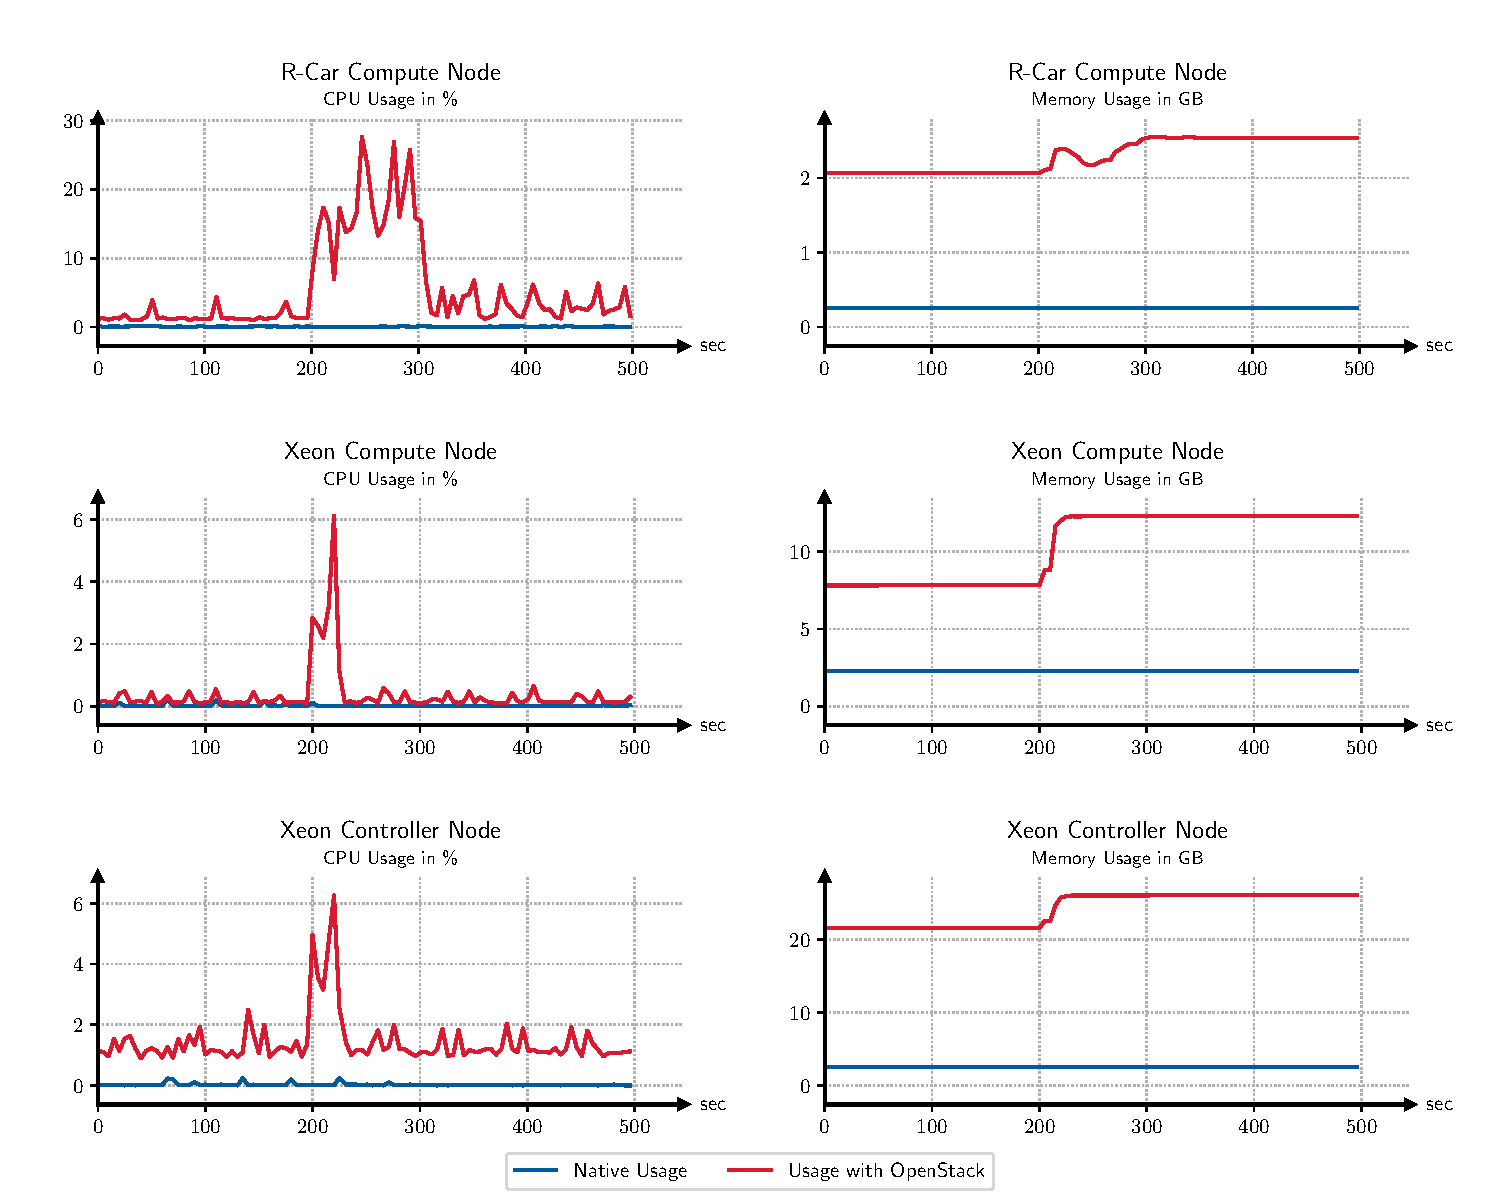
\includegraphics[width=\linewidth]{05_all-startup.pdf}
          \captionof{figure}{Idle CPU and memory usage on all tested platforms}
          \label{fig:all_idle}
        \end{figure}
        
        \newpage
        \noindent According to Section \ref{section:methodology_idle}, the CPU and memory usage is measured on a system with and without active OpenStack services.
        The goal is to examine the overhead introduced by solely running OpenStack services and provisioning one \ac{VM}.
        For all systems, a baseline measurement is performed to enable the comparison against the native system.
        Regarding the native CPU usage, all platforms have a nearly 0\% CPU usage due to being a fresh installation with no active services.
        As for the native memory usage, with 400 MB the R-Car node has clearly a smaller memory usage than the Xeon nodes. 
        This is expected because of the R-Car's custom kernel with an Ubuntu 18.04 Base \ac{OS}, contrary to the Xeon's full Ubuntu 18.04 Server \ac{OS} and standard Linux kernel.
        As expected, both Xeon nodes have similar memory usage of about 2.5 GB running without OpenStack.        
        
        \noindent Installing OpenStack on all R-Car and Xeon nodes (see Figure \ref{figure:network_setup}) indeed introduces overhead on the \ac{CPU} and memory.
        Clearly visible, the OpenStack services introduce on all platforms small periodic peaks.
        These are due to OpenStacks's periodic services, which poll information from all compute hosts.
        Starting the scenario described in Section \ref{section:methodology_idle}, the first 200 seconds in each plot in Figure \ref{fig:all_idle} show the resource usage for all services running in an idle state and a configured but turned-off VM.
        On the R-Car compute node, the \ac{CPU} usage increases by 2\% on average, while on the Xeon compute node, it increases by only 0.3\% compared to the native usage.
        This is due to the much higher core number and higher performance of the Xeon CPU, leading to an overall lower impact of the additional services. 
        On the other hand, on the Xeon controller node, the \ac{CPU} usage increases significantly by about 1\%.
        The significant increase compared to the Xeon compute node depicts the additional core services running the controller node.
        This threefold increase in CPU usage versus the Xeon compute node indicates that all controller services are about two times as heavy as the compute services.
        Continuing with the \ac{VM}'s startup after 200 seconds, it is visible that the R-Car requires much more \ac{CPU} power to perform the startup.
        Also, the longer-lasting \ac{CPU} usage increase shows that the startup takes about four times longer on the R-Car node than on the Xeon nodes.
        Compared to the scenario with a turned-off VM (first 200 seconds), an active but idle VM only impacts the \ac{CPU} usage on the R-Car node.
        After ca. 225 seconds on the Xeon nodes, the VM started successfully and runs in an idle state, introducing no visible overhead compared to a turned-off VM.
        After ca. 310 seconds, the VM also started successfully on the R-Car but influences the CPU more visibly compared to a turned-off VM.
        Again the lower impact on the Xeon nodes can be attributed to the overall higher performance of those CPUs and the therefore smaller impact of more load.
        
        \noindent Considering memory usage, similar observations can be made.
        Compared to an idle system, the OpenStack services and the turned-off VM introduce an overhead of 1.8 GB (2.0 GB total)  on the R-Car and about 5 GB (7.5 GB total) on the Xeon compute node.
        Further, on the Xeon controller node, OpenStack requires additional 19 GB of memory (21,5 GB total) to provide all core and compute services.
        Assuming the compute services behave similarly as on the Xeon compute node, all controller services require about 14 GB of additional memory, making them about three times as heavy as the compute services.
        However, these memory values are influenced by the yet turned-off \ac{VM}.
        Measuring the memory usage without any \ac{VM}, the R-Car shows a total memory usage of 900 MB, while the Xeon compute and controller nodes show a total usage of 3.1 GB and 13 GB.
        This corresponds to an overhead of about 400-500 MB on the compute nodes and about 13 GB on the controller node solely through the OpenStack services..
        Starting the \ac{VM} increases the memory usage on all platforms.
        An increase of about 400 MB is measured on the R-Car node, and the Xeon nodes require an additional 4 GB for the \ac{VM} provisioning. 
        Once the \ac{VM} is booted successfully, the memory usage does not change due to the \ac{VM} also being in an idle state without any running services inside.
        The higher memory required by the Xeon nodes correlates to the higher \ac{VM} memory configuration.
        Starting a VM with a lower memory configuration reduces this memory increase.
        
        \noindent Overall, the results confirm the introduction of overhead through OpenStack.
        However, an \ac{CPU} usage overhead of about 3-4\% on the R-Car nodes and especially of about 0.2\% on the Xeon compute node while provisioning \acp{VM} is lower than expected.
        An overhead in such dimensions does not rule OpenStack out on these systems.
        The same applies to memory usage. 
        Especially the lower memory usage on the R-Car nodes is interesting and suggests a more in-depth examination.
        The controller node requires more memory and more CPU performance due to the additional core services. 
        This advices to use a powerful enough system or dedicated network and storage nodes to provide the core services.
        The difference regarding both platforms' overhead originates from the high difference in computational performance and the chosen VM configurations.
        This makes the platforms not directly comparable but suggests considering them as possible low-end and high-end platforms.
        

    \section{OpenStack's Impact on Resources}
    \label{section:evaluation_performance}
        
        Examining the in Chapter \ref{chapter:methodology} defined resource's performance, the measurements show that all resources suffer some performance degradation.
        In all performed tests, the OpenStack \acp{VM} are outperformed by the native hardware.
        As expected, the R-Car node performs overall weaker than the Xeon nodes due to not being intended for such a use case and representing a low-end hardware.
        However, the impact on none resource is substantial enough to entirely exclude OpenStack on either the ARM or the x86 platform.
        The following sections present the measurements on every resource.
        
        \subsection{Effects on the CPU}
        \label{subsection:cpu_impact}
            
            \begin{figure}[ht]
              \centering
              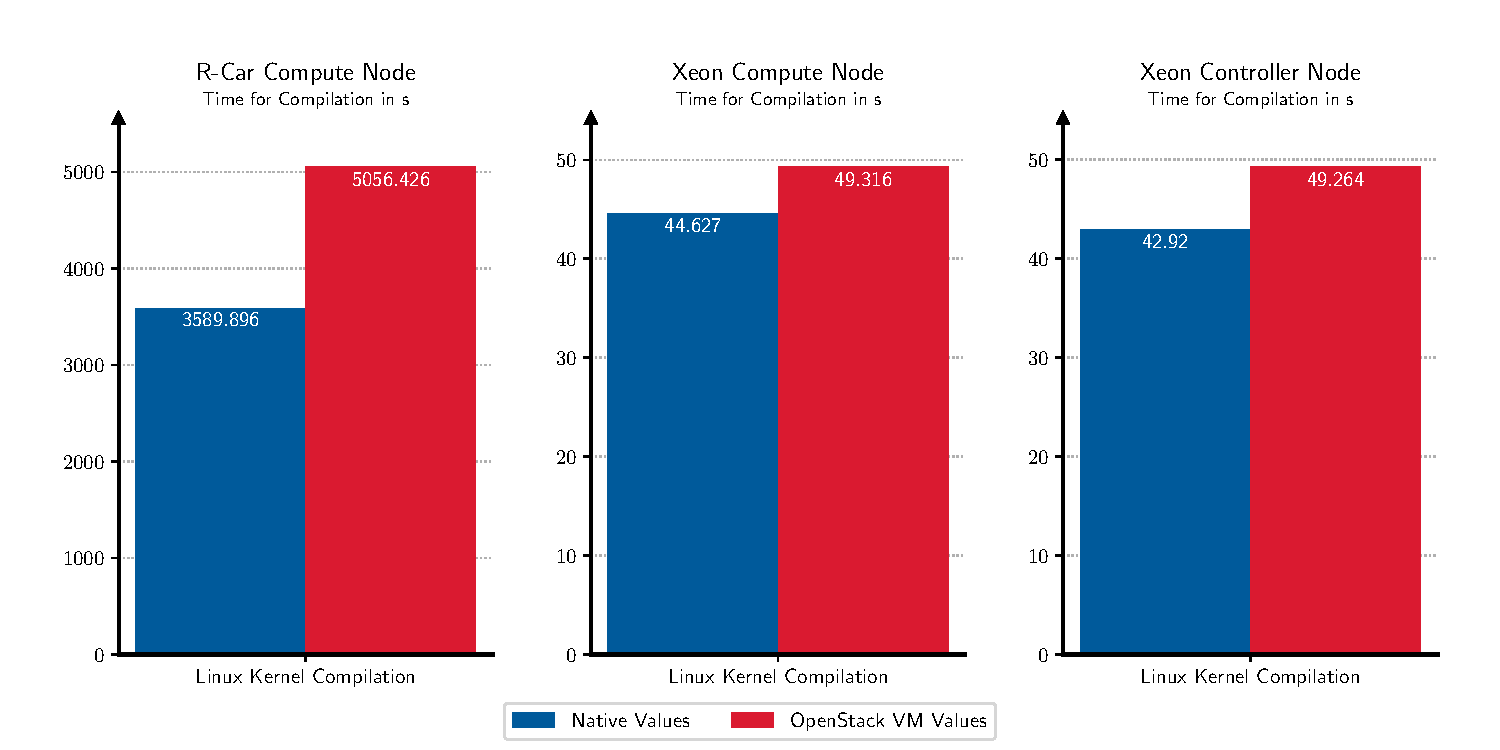
\includegraphics[width=\linewidth]{05_all-cpu.pdf}
              \captionof{figure}{Timed Linux Kernel compilation on all tested platforms}
              \label{fig:all_cpu}
            \end{figure}
            
            \noindent To evaluate the CPU performance degradation inside a VM, a Linux kernel compilation was chosen to stress the CPU, as explained in Section \ref{subsection:methodology_cpu}.
            Examining the difference in time between the native and the \ac{VM} compilation, a bigger difference is found on the R-Car node. 
            On the Xeon compute node, the \ac{VM} is about 4.7 seconds or 9.5\% slower, and on the Xeon controller node, it is about 6,3 seconds or 12.9\% slower.
            The weaker performance on the controller node is due to the additional services running and the, therefore, higher CPU load.
            Interestingly, both Xeon \acp{VM} perform nearly the same, with the difference being the native value, which is better on the controller node.
            However, a performance overhead of 10\% by the compute services on the compute node is tolerable.
            As the Xeon controller node in the here used configuration would represent the worst-case performance, an overhead of 13\% is also acceptable.
            
            \noindent The R-Car node, on the other hand, performs far worse.
            Comparing the \ac{VM} compilation versus the native compilation, the \ac{VM} takes about 1466 seconds or 29\% longer to compile the kernel.
            Introducing such performance degradation, OpenStack would not be usable on this hardware.
            The R-Car's high overhead is, on the one hand, due to the low core number and its big.LITTLE architecture, on the other hand, due to the R-Cars low secondary storage performance.
            As described in Chapter \ref{chapter:host_and_Test_setup}, the VM's cores are pinned to the host's high-performance cores.
            Through pinning the \acp{vCPU} to actual physical \ac{CPU} cores, the virtual processes are executed on predefined \acp{CPU} cores.
            Contrary to the Xeon nodes, this takes the ability to reschedule these tasks to other cores by the host \ac{OS}.
            Having enough cores to prevent a high utilization of one core, this should not impact the performance.
            However, the kernel compilation utilizes the full \ac{vCPU} and, therefore, all physical high-performance cores by 100\%.
            As the actual OpenStack compute services on the host also require computational power, they are simultaneously executed on the high-performance cores, leading to an over-utilization of those cores.
            This further leads to worse performance in general.
            Also, during the compilation process, many relatively small files need to be read from storage. 
            Due to the low secondary storage performance on the R-Car, found and discussed in Section \ref{subsection:disk_impact}, the results are further influenced and not 100\% representative.
            The R-Car results represent a worst-case scenario of a highly utilized CPU and low storage performance. 
                        
            \noindent Figures \ref{fig:two_threaded_host} and \ref{fig:two_threaded_vm} depict exemplary how a two-threaded instead of a four-threaded \ac{VM} task stresses the cores inside the \ac{VM} and on the actual host \ac{CPU}.
            Inside the VM, cores 1 and 2 are fully loaded, leading to also fully loaded cores 1 and 2 on the host itself.
            As only two threads are being used, cores 3 and 4 inside the VM are idle and barely used.
            However, despite the non-utilized VM cores, on the host the cores 3 and 4 show a usage of 20\% and 13\%, indicating that apart from the VM application OpenStack's compute services also require a certain amount of resources.
            
            \begin{figure}[ht]
            \centering
                \begin{subfigure}[b]{0.48\textwidth}
                    \centering
                    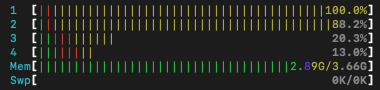
\includegraphics[width=\textwidth]{05_cpu-usage-rcar-compilation}
                    \caption{R-Car high performance cores utilization}
                    \label{fig:two_threaded_host}
                \end{subfigure}
                \hfill
                \begin{subfigure}[b]{0.48\textwidth}
                    \centering
                    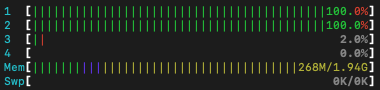
\includegraphics[width=\textwidth]{05_cpu-usage-vm-compilation}
                    \caption{VM cores utilization}
                    \label{fig:two_threaded_vm}
                \end{subfigure}
                \caption{Host and guest CPU utilization during a 2 threaded VM task}
                \label{fig:two_threaded_utilization}
            \end{figure}

            \noindent To gather better and more reliable insights, this test should be repeated first, on a broader range of hardware, and second, with a more precise configuration.
            The big.LITTLE architecture in this configuration of four high-efficiency and four high-performance cores is not ideal. 
            Through configuring, for example, the VM to used particular cores and the host to use other cores for the compute services, a mutual influence on each other could be prevented.
            Nevertheless, this would require hardware with sufficient computational power to provide sufficient resources to the host and the VM.
            Due to the over-utilization and deficient secondary storage performance, the results rather represent the worst-case. 
            However, through the better guest and host configuration regarding the utilized cores and better storage solutions, better and closer to reality results could be achieved.
           
        
        \subsection{Effects on the Secondary Storage}
        \label{subsection:disk_impact}
            
            \begin{figure}[ht]
              \centering
              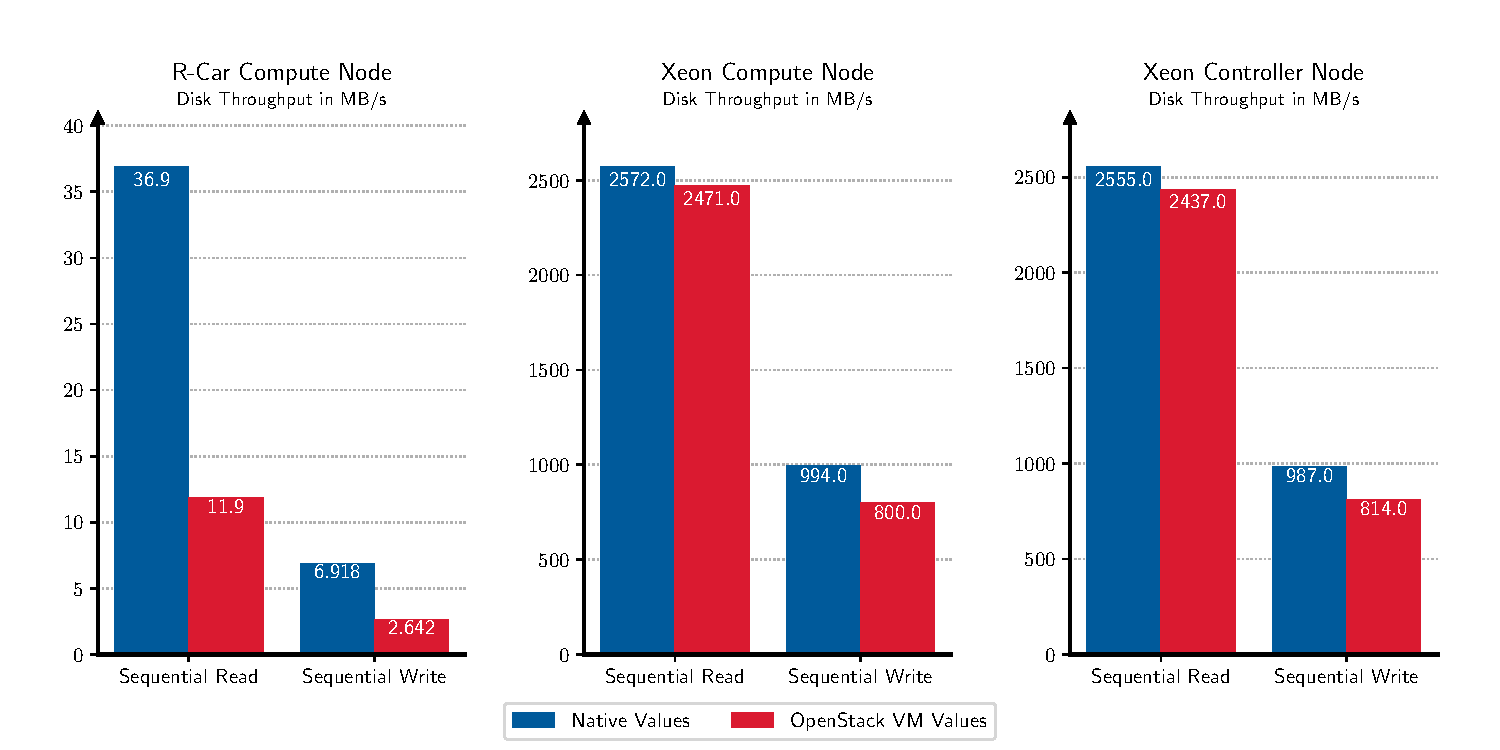
\includegraphics[width=\linewidth]{05_all-disk.pdf}
              \captionof{figure}{Storage performance on all tested platforms}
              \label{fig:all_disk}
            \end{figure} 

            \noindent As described in Section \ref{subsection:methodology_storage}, the platform's secondary storage's sequential read and write speeds were measured.
            Figure \ref{fig:all_disk} shows the native and \ac{VM} storage performance on all evaluated systems.
            Clearly visible, the R-Car has the worst performance in general and suffers the greatest performance impact.
            During testing, the SD-Card was found to achieve ambiguous results using different block sizes for testing. 
            Despite the SD-Card's general low performance, a block size of 128kb was found to deliver stable and consistent results.
            Inside the \ac{VM}, the storage suffers a 25 MB/s or 68\% performance impact regarding sequential read speeds.
            Also, sequential write speeds are impacted by 4 MB/s or 62\%.
            However, the measured values are not representative for two reasons.
            First, an SD-Card would not be used in a real-world scenario due to its low performance.
            Instead of SD-Cards, on-board storage like flash-storage or embedded multimedia cards would be used.
            The SD-Card was nevertheless chosen due to the easier handling regarding reflashing and reconfiguration of the host software.
            Second, because of the SD-Card's low performance, even little variation in performance yields a high percentage overhead.
            An impact of 25 MB/s on the Xeon platform would seem negligible, however, it makes a significant difference on the R-Car platform.
            Further tests using more suitable storage would very likely provide better and more accurate results.
            Especially the usage of the R-Cars' on-board flash storage would yield real-world values.
            However, this was not considered in this thesis due to the limited storage capacity of the on-board flash, the installation complexity using two partitions, and to preserve the \ac{SoC}'s flash of numerous reflashes.
            
            \noindent In contrast, the Xeon nodes feature an NVMe drive, enabling better insides on this platform.
            As the plots in Figure \ref{fig:all_disk} show, the performance is significantly better on native and virtual hardware.
            Both Xeon nodes show similar performance impacts.
            Regarding sequential read speeds, the \acp{VM} suffer a 100-128 MB/s or 4-5\% impact, while at sequential write speeds, the \acp{VM} suffer a 173-194 MB/s or 18-20\% impact.
            Commonly, write speeds are lower than reading speeds due to the actual process of changing and physically writing data to the storage device.  
            The low performance degradation regarding sequential read speed presents an acceptable overhead.
            However, the impact regarding the sequential write speeds is significant and not neglectable.
            
            \noindent Despite the bad results on the ARM platform and the high overhead for sequential writes on the x86 platform, the results have to be relativized.
            In an automotive embedded environment, apart from research with many measurements creating lots of data points, the data to be stored and read is relatively small.
            This makes full utilization of the available bandwidth unlikely.
            Further, the read speeds are more relevant and ensure a fast execution of applications, which is desirable and achieved by the x86 platforms.
            The x86 platform also depicts that OpenStack is capable of utilizing high-speed storage.
            The performance could be further increased utilizing OpenStack's object storage service \textsl{Swift} or enhancing the configuration towards storage performance.
            Also, a real-word test scenario would provide better reliability regarding the results.

           
        \subsection{Effects on the Memory}
        \label{subsection:memory_impact}
            
            \begin{figure}[ht]
              \centering
              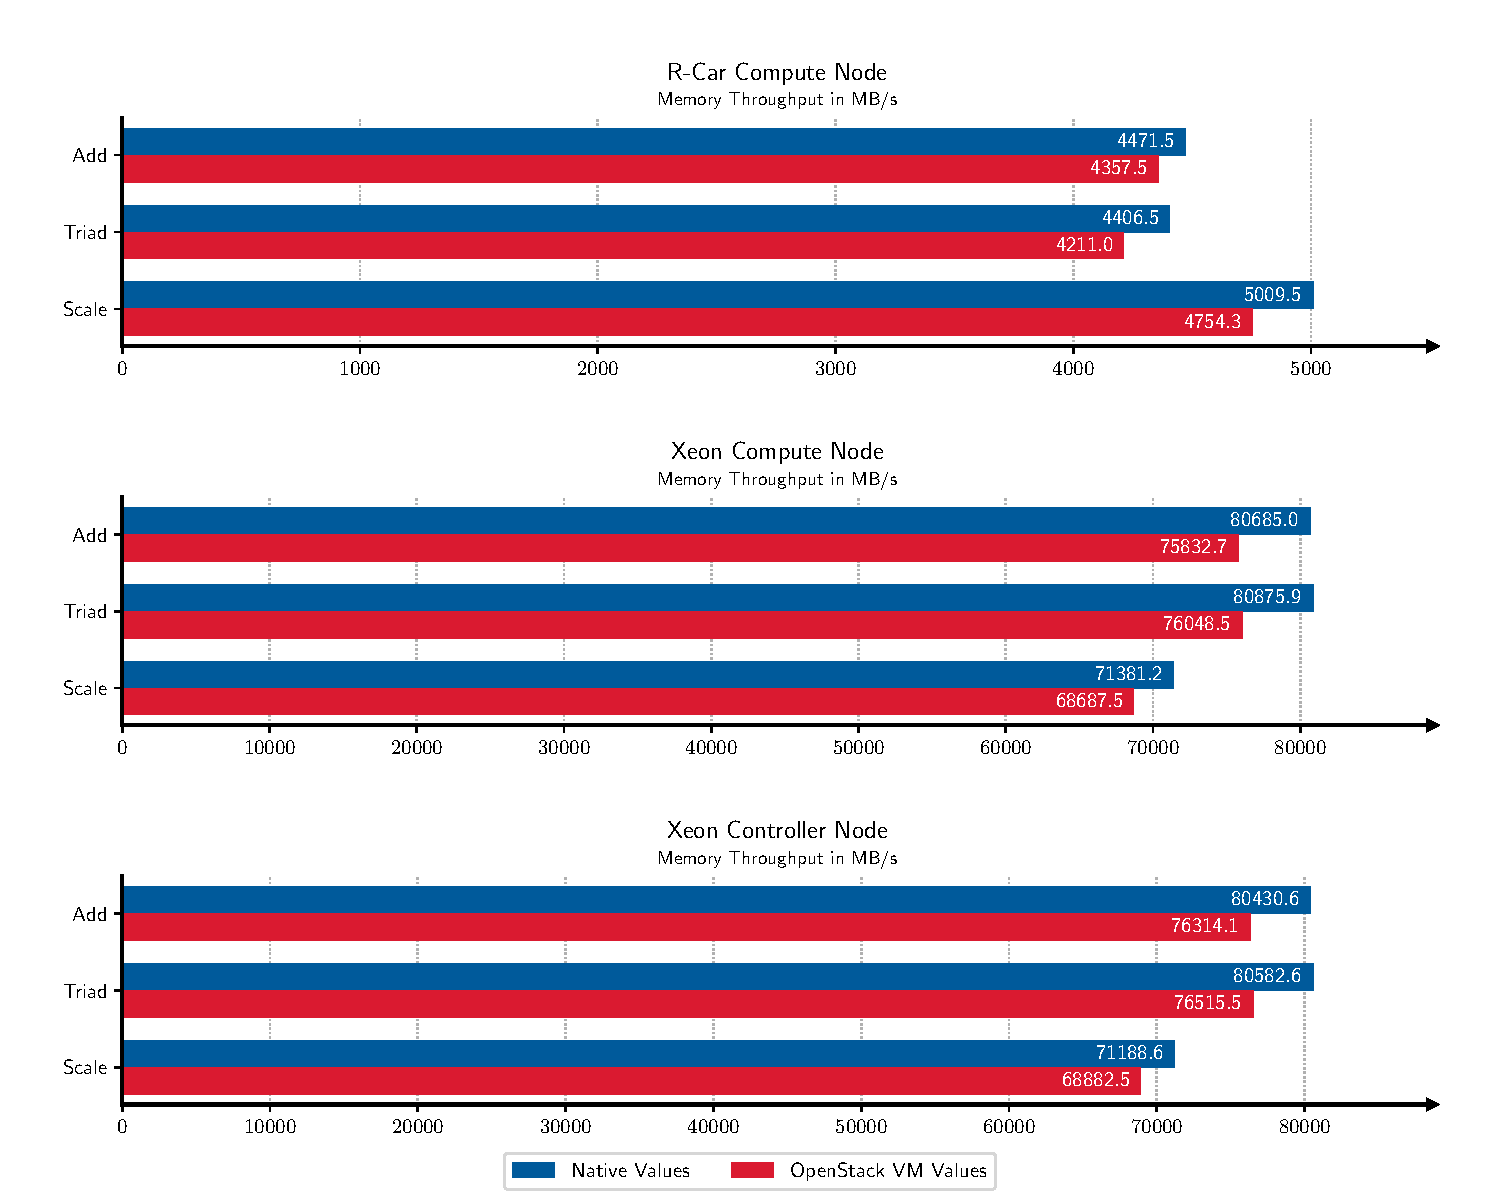
\includegraphics[width=\linewidth]{05_all-mem.pdf}
              \captionof{figure}{Memory throughput on all tested platforms}
              \label{fig:all_mem}
            \end{figure}
            
            \noindent Having measured the memory performance through mathematical operations according to Chapter \ref{subsection:methodology_storage}, Figure \ref{fig:all_mem} depicts the results.
            All \ac{VM} measurements are lower than the native ones.
            Due to being processed by more software layers compared to a native operation, \ac{VM} operations must be lower than native operations.
            The significantly higher throughputs on the Xeon systems reflect the higher thread count used on the Xeon nodes.
            However, dividing the values by the thread number yields values in pretty similar dimensions.
            
            \noindent On the R-Car node, OpenStack introduces an overhead of 3\% (add), 4\% (triad) and 5\% (scale).
            On the Xeon nodes, the introduced overhead lies in the same area at 3-6\%.
            Contrary to the R-Car node, the Xeon nodes' scale operation introduces a lower overhead of 3\% compared to the R-Car, where an overhead of 5\% is introduced.
            However, the native performance of the Xeon nodes' scale operation is in general lower compared to the two other operations, while on the R-Car, it is higher.
            This suggests that the ARM platform natively better supports such operations compared to the x86 platform.
            
            \noindent Overall, an overhead of 3-6\% on both platforms is plausible and acceptable. 
            This indicates excellent computational performance with little performance degradation. 
            Also, despite the R-Car's small memory, the performance is not impacted, further indicating good performance on systems with lower memory. 


        \subsection{Effects on the Network}
        \label{subsection:network_impact}
            
            \begin{figure}[ht]
              \centering
              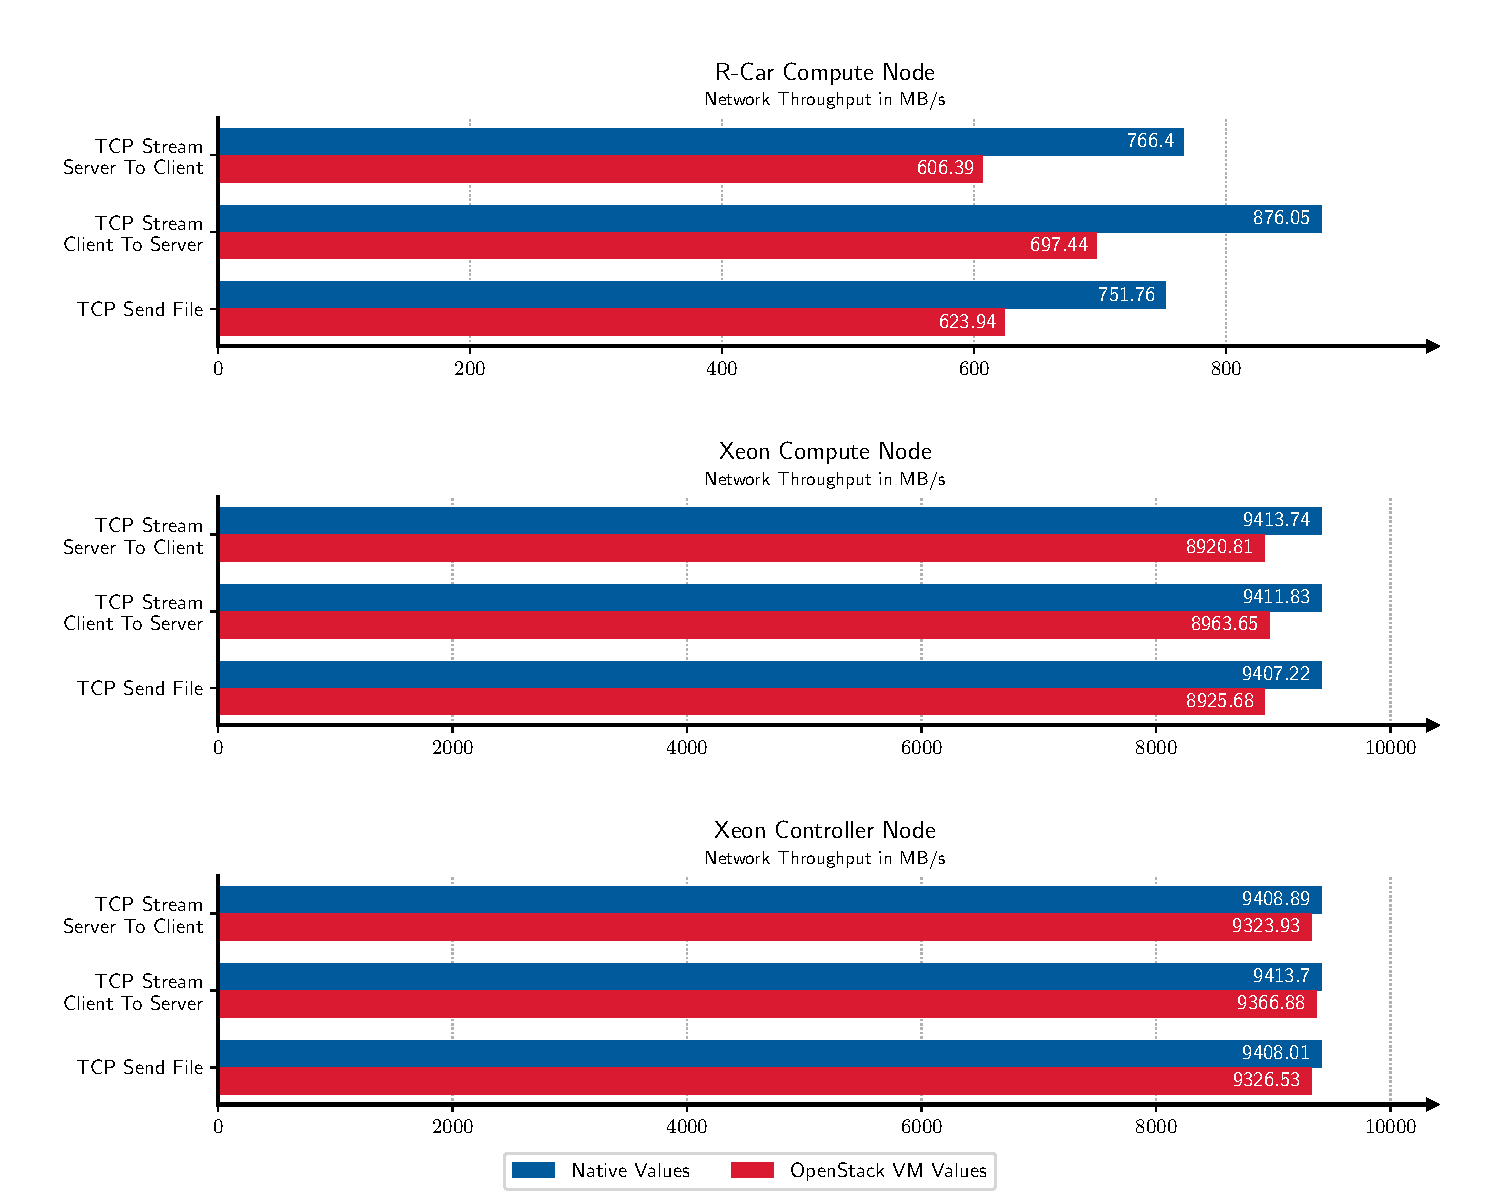
\includegraphics[width=\linewidth]{05_all-net.pdf}
              \captionof{figure}{Network throughput on all tested platforms}
              \label{fig:all_net}
            \end{figure}
            
            \noindent Studying the network throughput results in Figure \ref{fig:all_net}, all three tested platforms yield different results.
            First, the Xeon nodes yield much higher general performance due to their 10 Gbit connection.
            This already is a relevant finding as modern vehicles make more and more use of 1 Gbit and, in the future, probably 10 Gbit connections.
            The performed measurements show that OpenStack can handle these connections.
            On the other hand, the R-Car node is only equipped with a 1 Gbit network interface, yielding significantly lower results.
            
            \noindent The overhead lies at 20\% for the stream tests on the R-Car node and at 17\% for the file send test. 
            In all tests, the VM suffers a similar impact, which could be related to the R-Car's overall lower computing capabilities during the simultaneous usage of the high-performance cores by the host and guest.
            As described in \ref{subsection:cpu_impact}, the simultaneous resource usage by host and guest requires additional computational resources, as well as time, which reduces the throughput.
            In the context of network performance, additional services process data-packets before actually releasing them onto the network and vice versa.
            
            \noindent Examining the Xeon compute node, results with much lower overhead are found.
            For all tested connections, the overhead stays at about 5\%.
            This strengthens the indication that the host system's computational capabilities can influence network performance and lead to better results.
            Also, the results show that the VM utilizes the hardware and the 10 Gbit connection used. 
            
            \noindent Closing, the controller node delivers additional insides on the performance overhead.
            Regarding the test configuration, the environment differs in two points from the ones of the R-Car and the Xeon compute node.
            First, the compute services are now located on the same host as the OpenStack network service Neutron.
            This means that all requests can be directly processed by the same host and send out to the real world network without being first processed by a different node.
            Second, the Netperf-Server is now not being run on the controller node but on the Xeon compute node, making the controller node less utilized.
            This leads to an even lower overhead of only 1\% for all TCP connections.
            
            \noindent Considering the low and very low overheads of 5\% and 1\% on the Xeon nodes, the performance is again satisfactory.
            The Xeon controller node's performance raises the possibility of always executing the Neutron service and the Nova services along with each other.
            At the expense of other resources, this could provide nearly native performance if necessary.
            The significant overhead of 20\% on the R-Car, on the other hand, is not acceptable.
            However, in an automotive environment, the transferred data is relatively small, containing small pieces of information like signals.
            Therefore, high throughput rates might not always be the primary concern, but rather the latency.
            However, as with storage, OpenStack enables various network configurations and enhancements, which would improve network performance.
            In addition, the usage of an ARM platform with 10 Gbit Ethernet and higher computational power would most likely increase the comparability and reliability of the results.
            
            \begin{figure}[ht]
              \centering
              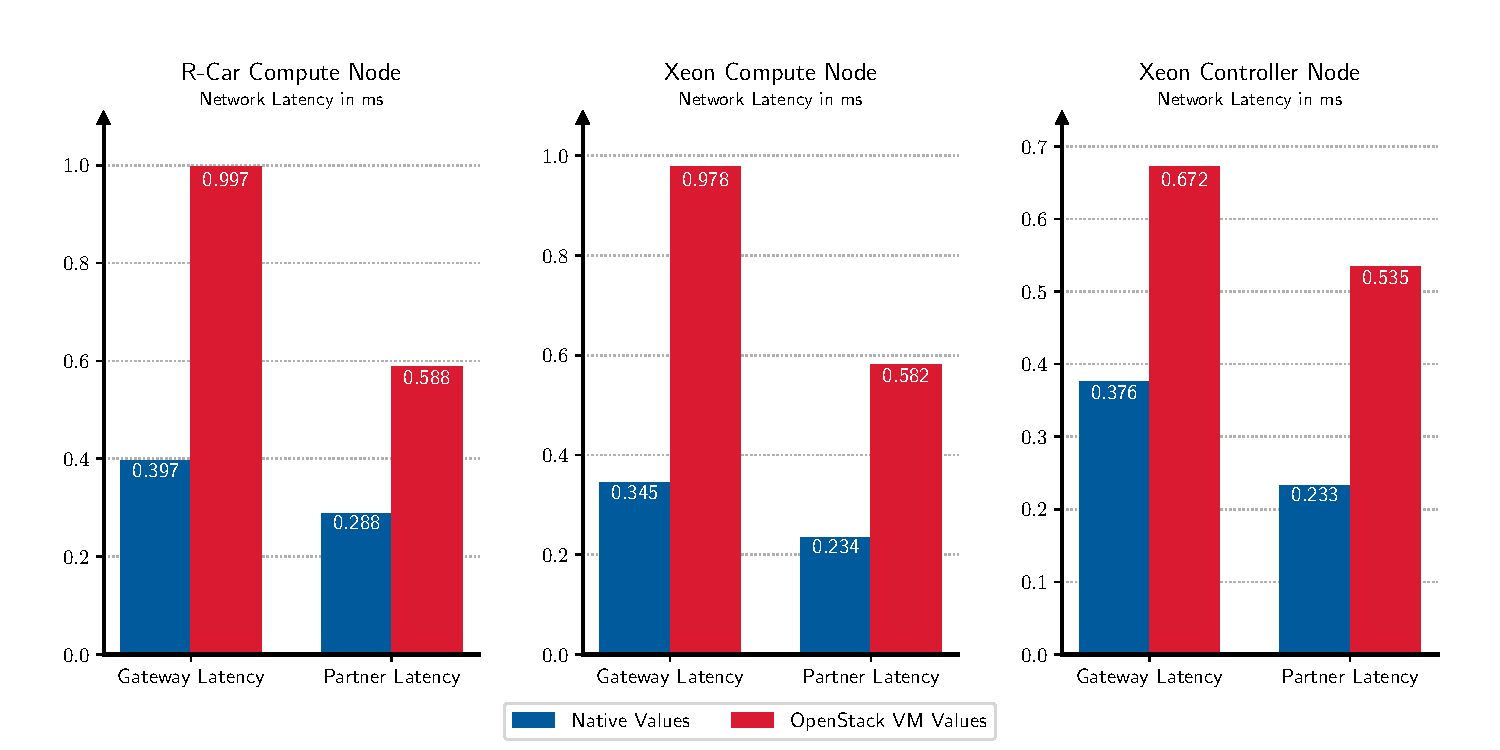
\includegraphics[width=\linewidth]{05_all-net-ping.pdf}
              \captionof{figure}{Network latency on all tested platforms}
              \label{fig:all_net_ping}
            \end{figure}
            
            \noindent Despite the different hardware and platforms, all performed latency tests yield very similar results in Figure \ref{fig:all_net_ping}.
            Pinging the gateway, a host not part of the OpenStack cluster, results in a latency measurement between 0.35 and 0.4 milliseconds.
            Pinging the Xeon controller and the Xeon compute node, hosts part of the OpenStack cluster, yields times about one millisecond shorter.
            This is accountable to the higher performance of the nodes versus the lower performance of the gateway.
            
            \noindent Regarding the measurements from inside the \ac{VM}, a clear overhead can be identified.
            Pinging the gateway, the R-Car, and the Xeon compute node yield a latency of about three times as high as natively.
            The Xeon controller node yields a latency of two times as high as natively.
            This overhead of about 200\% and 100\% can be attributed to the way OpenStack routes packets, in this case, ICMP packets, to their destination.
            Until the packets are released onto the real-world network, they are routed on an internal OpenStack network to the Neutron service host, in this case, the Xeon controller node.
            Arrived at the network node, the packets are processed by Neutron and only then released onto the real-wold network.
            The same situation applies to the replies in the backward direction.
            
            \noindent Executing the ping from the Xeon controller node VM gives the possibility to identify OpenStack's actual overhead.
            Because the controller VM packets are already on the controller hardware, only an one-time processing of them is necessary to place the packets on the real-world network.
            Taking 0.3 milliseconds more on the controller node for both pings, this 0.3 milliseconds are the actual overhead introduced by OpenStack.
            This also matches the fact that the overhead is twice as high with 0.6 milliseconds on the two compute nodes, as on those nodes, the packets have to be processed twice, on the compute host itself and on the network node.
            Considering further that the ping utility measures the round trip time, meaning from source to destination and back, the actual overhead is even smaller.
            OpenStack introduces an overhead of about 0.15 milliseconds from the Neutron service host and 0.3 milliseconds from other compute hosts for packets to reach their destination. 
            
            \noindent Considering the native values, 100\% and 200\% longer latency values are not negligible.
            Nevertheless, the measurements were performed on a local network and within a close range. 
            Real-world networks could introduce much longer latencies, making the native values much bigger.
            For example, a ping to the Google DNS server takes about 15 milliseconds.
            Considering an overhead of 0.3 or 0.6 milliseconds from an OpenStack \ac{VM}, the percentage overhead is only 2\% or 4\%, being well reasonable and acceptable.
            Being an extreme example as the packets have to travel a long distance shows that the actual overhead compared to the native hardware can vary on a different network.
            To gather real-world values, the test should be performed on an actual automotive network with a real-word load.

    \section{Summary}
    \label{section:summary}
        
        Concluding from the performed results, OpenStack clearly introduces an overhead in all considered domains.
        However, on both evaluated platforms, the VMs function consistently and reliably. 
        
        \noindent The Xeon systems represent a significantly more powerful embedded platform which delivers very high performance.
        OpenStack's impact on this platform is relatively small, and little performance degradation is measured. 
        This suggests an actual in-vehicle use.
        The R-Car results, in contrast, do not show such good performance.
        Considering the high performance degradation of the CPU and secondary storage, an in-vehicle use seems not promising.
        However, the network and memory performance measurements show that good performance is achievable on the R-Car and the degradation does not apply generally.
        This promises better and improved performance on different hardware with better components like faster secondary storage and more CPU cores.
        
        \noindent Despite the overhead, all functionality is continuously available, enabling the consideration of OpenStack's advantages in the following chapter.
        This chapter identified and evaluated the major negative impacts and disadvantages of OpenStack: the overhead and performance degradation.
        However, neither the better nor the worse performance of the platforms used do entirely prevent further tests or the in-vehicle usage in general. 
